% Historical appendix; not included in the current report.
\section{Controlled-budget recurrent execution}
\label{app:recurrent}
This auxiliary experiment isolates paging under an imposed allocation budget,
rather than demonstrating physical device-capacity scaling. The archived
configuration uses 32,768, 131,072 and 524,288 nodes, 16 periodic source offsets
per destination and four FP32 features. Topology and source fields are persisted
before execution. Neighbor averaging is applied ten times, with each output
becoming the next input; an independent NumPy oracle checks every step.

Full materialization (\emph{resident}), 1,024-row pages and 8,192-row pages each
run in three fresh processes under a 24 MiB native GPU-buffer budget. Here
resident means that the complete CSR and input field are loaded into GPU
memory before computation. Graph loading and the first forward are separate;
warm timing uses steps 2--10. Measured forward includes synchronous computation,
page reads and host/device staging, but excludes oracle checking and explicit
between-step garbage collection. Memory checkpoints follow that collection.
These are forward-call costs, not uninterrupted iteration throughput.

\begin{figure}[htbp]
\centering
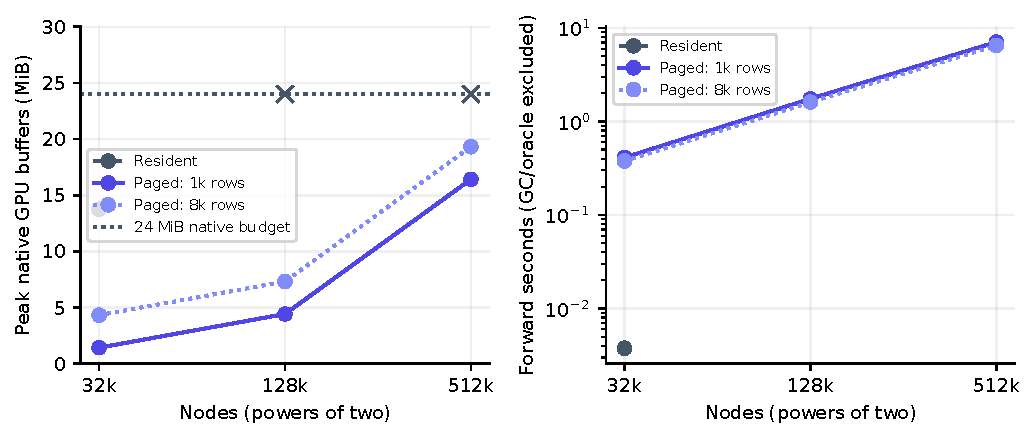
\includegraphics[width=\linewidth]{figures/gpu-paged-capacity.pdf}
\caption{Auxiliary CUDA paging experiment under a 24 MiB native-buffer budget.
Crosses mark rejected full-residency configurations, not measured 24 MiB peaks.
Forward time is the median of three process-level warm medians.}
\label{fig:cuda-capacity}
\end{figure}

The largest graph contains 8,388,608 edges and about 76 MiB of stored data.
Both page choices complete all ten steps in every trial. The 1k-row path peaks
at 16.41 MiB of tracked GPU buffers and retains an 8 MiB output after collection.
The resident path is rejected by the imposed budget, not physical device memory.

\begin{figure}[htbp]
\centering
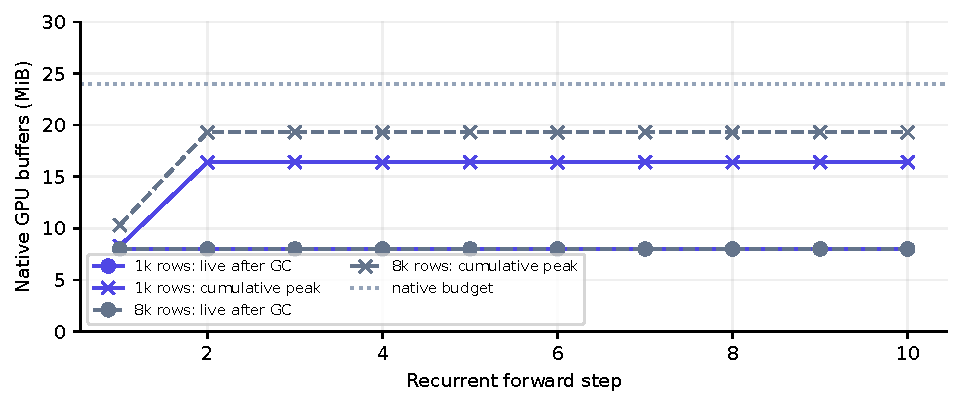
\includegraphics[width=.94\linewidth]{figures/gpu-paged-iterations.pdf}
\caption{Ten recurrent steps at 524,288 nodes. Live-output checkpoints coincide
at 8 MiB; the other curves are cumulative managed allocation peaks. Accounting
excludes CUDA/compiler pools, existing services, Python objects and OS page cache.}
\end{figure}

These archived runs use host collection of page outputs before final assembly;
the billion-edge runs use the incremental assembly described in
Section~\ref{sec:gpu-paging}. Their source hashes and measurement protocols remain
separate. The smaller experiment establishes only the checked ten-step behavior,
not long-term leak freedom or billion-edge training. CUDA paged backward,
automatic byte-budget-derived page selection and asynchronous I/O overlap are
not evaluated. Raw records and validation scripts reside in \code{data/runtime/}.
\FloatBarrier
